\documentclass[10pt, twoside, a4paper, openright]{report}

%packages-----------------------------------------------------------------------

\usepackage[utf8]{inputenc}
\usepackage[english]{babel}
\usepackage[T1]{fontenc}
\usepackage{lmodern}
\usepackage{array}
%\usepackage{times}
%\usepackage{helvet}
%\usepackage{charter}
\usepackage{graphicx}
\usepackage{color}
\usepackage{amsmath}
\usepackage{amssymb}
\usepackage{amsthm}
\usepackage{verbatim}
\usepackage{pdfpages}
\usepackage[unicode]{hyperref}
\hypersetup{
	colorlinks=true,
	urlcolor=blue,
	linkcolor=blue,
	citecolor=blue
}
\newcommand{\link}[3][blue]{\href{#2}{\color{#1}{#3}}}%
\usepackage[small, bf]{caption}
\usepackage{enumerate}
\usepackage{epstopdf}
\usepackage{epsfig}
\usepackage{setspace}
\usepackage{esdiff}
\usepackage{enumitem}
\usepackage[inner=4.0cm, outer=3.0cm]{geometry}
\usepackage{emptypage}
\usepackage{caption}
%\usepackage{subcaption}
\usepackage{listings}
\usepackage{multicol}
\usepackage{multirow}
\usepackage{lipsum}
\usepackage{mathabx}
\usepackage{floatrow}
\usepackage{courier}
\usepackage{cite}
\def\citepunct{; \penalty\citepunctpenalty}
\usepackage[position=top]{subfig}
%\usepackage[autostyle]{csquotes}
\usepackage{microtype}

%\renewcommand{\familydefault}{\sfdefault}



\newcommand{\q}[1]{``#1''} % quotation marks

%cite----------



%fancystyles--------------------------------------------------------------------

\usepackage{fancyhdr}

\fancypagestyle{myfancy}{

\fancyhead[LE]{\nouppercase{\leftmark}}
\fancyhead[LO]{}
\fancyhead[CO]{}
\fancyhead[CE]{}
\fancyhead[RE]{}
\fancyhead[RO]{\nouppercase{\rightmark}}

\fancyfoot[LE]{\thepage}
\fancyfoot[LO]{}
\fancyfoot[CO]{}
\fancyfoot[CE]{}
\fancyfoot[RE]{}
\fancyfoot[RO]{\thepage}

\renewcommand{\headrulewidth}{0.4pt}
\renewcommand{\footrulewidth}{0.0pt}
}

\fancypagestyle{plain}{

\fancyhead[LE]{}
\fancyhead[LO]{}
\fancyhead[CO]{}
\fancyhead[CE]{}
\fancyhead[RE]{}
\fancyhead[RO]{}

\fancyfoot[LE]{\thepage}
\fancyfoot[LO]{}
\fancyfoot[CO]{}
\fancyfoot[CE]{}
\fancyfoot[RE]{}
\fancyfoot[RO]{\thepage}

\renewcommand{\headrulewidth}{0.0pt}
\renewcommand{\footrulewidth}{0.0pt}
}

%tikz---------------------------------------------------------------------------

\usepackage{tikz}
\usetikzlibrary{shapes, arrows}

%url----------------------------------------------------------------------------

\usepackage{url}
\DeclareUrlCommand\url{\def\UrlLeft{<}\def\UrlRight{>} \urlstyle{tt}}

%color--------------------------------------------------------------------------

\definecolor{darkred}{rgb}{0.6,0,0}
\definecolor{darkgreen}{rgb}{0,0.6,0}
\definecolor{darkblue}{rgb}{0,0,0.6}
\definecolor{darkgrey}{rgb}{0.3,0.3,0.3}
\definecolor{grey}{rgb}{0.6,0.6,0.6}
\definecolor{lightgrey}{rgb}{0.95,0.95,0.95}
\definecolor{lightred}{rgb}{0.99,0.85,0.85}
\definecolor{violet}{rgb}{0.65,0.45,0.75}

%listings-----------------------------------------------------------------------

\definecolor{mygreen}{rgb}{0,0.6,0}
\definecolor{mygray}{rgb}{0.5,0.5,0.5}
\definecolor{light}{rgb}{0.96, 0.96, 0.96}
\definecolor{mymauve}{rgb}{0.58,0,0.82}

\lstdefinestyle{CXX} {
	language=C++,
	backgroundcolor=\color{light},
	basicstyle=\scriptsize\ttfamily,
	breakatwhitespace=false,
	breaklines=true,
	captionpos=t,
	%commentstyle=\color{mygreen},
	deletekeywords={},
	escapeinside={\%*}{*)},
	extendedchars=true,
	frame=single,
	keepspaces=true,
	keywordstyle=\color{blue},
	otherkeywords={},
	numbers=left,
	numbersep=5pt,
	numberstyle=\tiny\color{mygray},
	rulecolor=\color{black},
	showspaces=false,
	showstringspaces=false, 
	showtabs=false,
	stepnumber=1,
	stringstyle=\color{mymauve},
	tabsize=3,
	title=\lstname   
}

\lstdefinestyle{FORTRAN} {
	language=[90]Fortran,
	backgroundcolor=\color{light},
	basicstyle=\scriptsize\ttfamily,
	keywordstyle=\color{blue},
	%commentstyle=\color{mygreen},
	breakatwhitespace=false,
	breaklines=true,
	captionpos=t,
	deletekeywords={},
	escapeinside={\%*}{*)},
	extendedchars=true,
	frame=single,
	keepspaces=true,
	otherkeywords={},
	numbers=left,
	numbersep=5pt,
	numberstyle=\tiny\color{mygray},
	rulecolor=\color{black},
	showspaces=false,
	showstringspaces=false, 
	showtabs=false,
	stepnumber=1,
	stringstyle=\color{mymauve},
	tabsize=3,
	title=\lstname 
}

%settings-----------------------------------------------------------------------

\setlength{\parindent}{15pt}
\setlength{\parskip}{0pt}
\renewcommand{\baselinestretch}{1.0}
\pagenumbering{arabic}
\frenchspacing

\DeclareFontFamily{U}{mathx}{\hyphenchar\font45}
\DeclareFontShape{U}{mathx}{m}{n}{<-> mathx10}{}
\DeclareSymbolFont{mathx}{U}{mathx}{m}{n}
\DeclareMathAccent{\widebar}{0}{mathx}{"73}

%commands----------------------------------------------------------------------

\newcommand{\ctu}{Czech Technical University in Prague}
\newcommand{\fnspe}{Faculty of Nuclear Sciences and Physical Engineering}
\newcommand{\dpe}{Department of Physical Electronics}
\newcommand{\branch}{Computational Physics}
\newcommand{\projecttitle}{Laser-driven sources of~electrons and~x-rays in~underdense plasma: theory and~simulation}
\newcommand{\projecttitlecz}{Laserem řízené zdroje elektronů a~rentgenového záření v~podkritickém plazmatu: teorie a~simulace}
\newcommand{\valenta}{Ing. Petr Valenta}
\newcommand{\klimo}{doc. Ing. Ondřej Klimo, Ph.D.}
\newcommand{\bulanov}{Prof. Sergei Vladimirovich Bulanov}
%\newcommand{\year}{2022}
\newcommand{\keywords}{}
\newcommand{\keywordscz}{}

%macros-------------------------------------------------------------------------

\newcommand{\nucl}[3]{
\ensuremath{
\phantom{
\ensuremath{^{#1}_{#2}}}
\llap{\ensuremath{^{\rule{0pt}{0pt}#1}}}
\llap{\ensuremath{_{\rule{0pt}{7pt}#2}}}
\mbox{#3}}}

\newcommand{\norm}[1]{\lVert#1\rVert}
\newcommand{\abs}[1]{\lvert#1\rvert}

\renewcommand{\vec}[1]{\mathbf{#1}}

\newcommand{\rot}[1]{\nabla \times #1}
\newcommand{\grad}[1]{\nabla #1}
\renewcommand{\div}[1]{\nabla \cdot #1}
\newcommand{\laplace}[1]{\Delta #1}
\newcommand{\dalembert}[1]{\Box #1}

\newcommand{\e}[0]{\mathrm{e}}
\renewcommand{\i}[0]{\mathrm{i}}
\renewcommand{\d}[0]{\mathrm{d}}

%changecountering---------------------------------------------------------------

\usepackage{chngcntr}
%\counterwithout{equation}{chapter}
\counterwithout{figure}{chapter}
\counterwithout{table}{chapter}

%document-----------------------------------------------------------------------

\begin{document}

\pagestyle{empty}

%1------------------------------------------------------------------------------

\mbox{}
\newpage

\begin{titlepage}

\begin{center}
\epsfysize=35mm \epsffile{img/logo/ctu.pdf} \\[15mm]
\end{center}

\begin{center}
\begin{spacing}{2.0}
{\rule{125mm}{2pt}} \\[4mm]
{\huge \bf \projecttitle} \\
{\rule{125mm}{2pt}} \\[5mm]
\end{spacing}
{\LARGE by Petr Valenta} \\
\end{center}

\vfill

\begin{center}
\parbox{0.75\textwidth}{\noindent \centering \large Dissertation submitted to the \\ \fnspe, \\ \ctu, \\ in partial fulfillment of the requirements for the degree of Doctor of Philosophy.}
\end{center}

\vfill

\begin{center}
{\large Prague, 2022}
\end{center}

\end{titlepage}

%2------------------------------------------------------------------------------

\newpage
\rule{0pt}{0pt}
\vfill
\begin{description}
	\item[supervisor:]\ \\
	\klimo \\
	\fnspe, \\ 
	\ctu, \\
	Břehová 7, 115 19 Prague, \\
	Czech Republic
\end{description}

\begin{description}
	\item[supervisor specialist:]\ \\
	\bulanov \\
	Institute of Physics, \\
	Czech Academy of Sciences, \\
	Na Slovance 1999/2, 182 21 Prague, \\
	%Za Radnicí 835, 252 41 Dolní Břežany, \\
	Czech Republic
\end{description}
\vglue 1cm

\noindent Copyright {\copyright} {2022} {Petr Valenta}

%3------------------------------------------------------------------------------

%\newpage
%\includepdf[pages=1]{dat/guidelines.pdf}

%4------------------------------------------------------------------------------

%\newpage
%\includepdf[pages=2]{dat/guidelines.pdf}

%5------------------------------------------------------------------------------

%\newpage
%\null
%\vfill
%{\bf \noindent Prohlášení/Declaration} \\[5mm]
%Prohlašuji, že jsem předloženou práci vypracoval samostatně a že jsem uvedl veškerou
%použitou literaturu.\\[2mm]
%I hereby declare that I carried out this work independently, and only with the cited sources, literature and other professional sources.\\
%\vspace{5mm}V Praze dne/In Prague on .............................\hfill
%\begin{tabular}{c}
%........................................\\
%\valenta
%\end{tabular}

%6------------------------------------------------------------------------------

%\newpage
%\thispagestyle{empty}
%\mbox{}

%7------------------------------------------------------------------------------

%\newpage
%\begin{flushleft}
%	\renewcommand{\arraystretch}{1.3}
%	\begin{tabular}{r p{12cm}}
%		Název práce:
%		~ & \bf \projecttitlecz \\
%		Autor:
%		~ & \valenta \\
%		Druh práce:
%		~ & Diplomová práce \\
%		Studijní program:
%		~ & (N3913) Aplikace přírodních věd \\
%		Obor:
%		~ & (3901T065) Informatická fyzika \\
%		Vedoucí práce:
%		~ & \klimo \newline Katedra fyzikální elektroniky, Fakulta jaderná a fyzikálně inženýrská, České vysoké učení technické v Praze \\
%		Konzultant:
%		~ & \bulanov \newline Projekt ELI-Beamlines, Fyzikální ústav Akademie věd České republiky, v. v. i. \\
%	\end{tabular}
%\end{flushleft}

%\begin{center}
%\textbf{Abstrakt}\\
%\end{center}

%Úzká fokusace s využitím plazmové optiky může vést ke zvýšení intenzity a zlepšení časového i prostorového kontrastu laserových svazků. Vzhledem k tomu, že pro popis těchto impulsů neplatí paraxiální aproximace, je zapotřebí použít vhodnější model. V rámci této práce byly do částicového kódu implementovány a důkladně otestovány nové okrajové podmínky pro výpočet časového vývoje laserového impulsu na hranici simulační obasti v souladu s Maxwellovými rovnicemi. Upravený kód byl použit pro simulace laserových svazků zaostřených do velmi malého ohniska. Výsledky simulací byly analyzovány z hlediska vlivu velikosti ohniska na průběh interakce laserových svazků s pevnými terči. Ukazuje se, že trajektorie horkých elektronů a absorpční procesy během interakce jsou silně ovlivněny příčnou složkou ponderomotorické síly, která je velmi vysoká v případě ohniska menšího než je vlnová délka laseru. V tomoto případě ostře narůstá účinnost absorpce laserové energie v plazmatu, distribuční funkce energie elektronů jsou kvalitativně rozdílné a teplota horkých elektronů se výrazně zvyšuje. \\

%\noindent Klíčová slova: \keywordscz


%8------------------------------------------------------------------------------

\newpage
\pagestyle{myfancy}

\chapter*{Abstract \markboth{Abstract}{Abstract}}
\addcontentsline{toc}{chapter}{Abstract}

%We explore novel regimes of laser-plasma interaction accessible by new generation laser systems. The scientific focus is mainly devoted to enhancement of laser-generated sources of accelerated electrons and coherent short-wavelength radiation based on plasma waves driven by intense laser pulses. First we describe mechanisms for obtaining electron beams based on laser wakefield acceleration technique. We analyze the properties of the wakefield in regimes dominated by the effects of dispersion and carrier envelope phase. Discussed range of parameters is relevant for electron acceleration at high repetition rate. Second we investigate the concept of relativistic mirrors in laser plasmas. We describe the recoil effects on reflection from relativistic mirrors which is crucial for maximizing the energy of reflected radiation. We find the threshold for incident pulse energy above which the relativistic mirrors undergo significant back reaction. We also analyze the generation of coherent hard electromagnetic radiation by the reflection from the electron density singularities.\\

{\noindent \bf Keywords:} laser-plasma interaction, laser-wakefield acceleration, relativistic mirrors, particle-in-cell simulation \keywords

\newpage
\thispagestyle{empty}
\mbox{}

%9------------------------------------------------------------------------------

\tableofcontents
\addtocontents{toc}{\protect\thispagestyle{empty}}
\thispagestyle{empty}

%-------------------------------------------------------------------------------

\chapter{Introduction}
%\addcontentsline{toc}{chapter}{Introduction}
%\input{dat/introduction.tex}

\section{Methods and state-of-the-art}

The operation of the world's first working laser was demonstrated by T. H. Maiman in 1960 \cite{Maiman1960}. Soon after, the introduction of Q-switching \cite{McClung1962} and mode-locking \cite{Mocker1965} enabled generation of laser pulses with GW peak power and sub-$ \mathrm{ps} $ duration. At the same time, most of the major effects in nonlinear optics were discovered or experimentally verified (e.g., generation of optical harmonics \cite{Franken1961}, optical rectification \cite{Bass1962}, optical Kerr effect \cite{Armstrong1962, Maker1964}, stimulated Raman scattering \cite{Woodbury1962}, stimulated Brilouin scattering \cite{Chiao1964b, Chiao1964}, multiphoton absorption and ionization \cite{Kaiser1961, Voronov1966}). 

Further amplification of laser pulses had been limited for a long time due to the development of nonlinear effects causing a detrimental pulse distortions or even a damage to the gain medium and optical components. This obstacle was overcome by applying the method of chirped pulse amplification \cite{Strickland1985, Maine1988} to optical amplifiers. To avoid the nonlinear effects, the laser pulse is stretched out temporally by several orders of magnitude (the input pulse energy is unchanged, but the intensity is lowered to an acceptable level) before passing through the amplifier medium and then compressed by the same ratio back to a duration similar to its initial value.

%\footnote{In 2018, G. Mourou and D. Strickland were awarded the Nobel Prize in Physics, for their joint work on chirped pulse amplification.}

A rapid progress in laser technology over several past decades has stimulated the development of high-power lasers all over the world. At the end of the 20th century, the laser pulses exceeded the PW power threshold \cite{Perry1999}. Currently, the highest laser pulse peak power achieved is 10 PW \cite{Tanaka2020}. Global efforts towards making the lasers even more powerful are continuing; historical perspective, current status, and future plans to attain the 100 PW level are summarized, e.g., in Refs.~\citenum{Danson2019} and \citenum{Li2021}.

Rather than power, however, it is often desired to reach the highest laser intensity (i.e., the power per unit area). The peak laser intensities can be increased either by further amplifying the laser beam energy or by reducing the size of the focal spot. While the former approach comes at great cost since it requires a higher level of complexity for the laser chain, the latter seems to be more effective due to the quadratic dependency of the laser intensity on the inverse of the focal spot radius. Therefore, a number of sophisticated focusing schemes have been under active investigation (e.g., multiple beam focusing \cite{Bulanov2010}, tight-focusing \cite{Bahk2004, Jeong2015}, $ 4 \pi $-spherical focusing \cite{Gonoskov2012, Jeong2020}). Recent experimental implementation of the tight-focusing scheme has demonstrated a record intensity over $ 10^{23} \ \mathrm{W / cm^{2}} $ by focusing a $ 4 \ \mathrm{PW} $ laser into a spot size of $ 1.1 \ \mathrm{\mu m} $ \cite{Yoon2021}.

Another very active research direction is to make the high-power laser pulses as short as possible. In the systems based on the chirped pulse amplification, the output pulse durations are inherently limited by the gain bandwidths of the amplifying media (e.g., the bandwidth of titanium-doped sapphire spans over $ \approx 75 \ \mathrm{nm} $, the obtainable bandwidth is further reduced by gain narrowing associated with amplification over several orders of magnitude \cite{Hotz1965}). Currently, there are two methods capable to tackle this issue: the optical parametric chirped pulse amplification \cite{Dubietis1992}, which extends the chirped pulse amplification technique by using the optical parametric amplifiers (i.e., amplifiers based on parametric nonlinear interactions), and the post-compression of laser pulses in large hollow-core fibers \cite{Nisoli1996}. The former method has recently demonstrated the generation of $ 5 \ \mathrm{PW} $, $ 18.6 \ \mathrm{fs} $ \cite{Zeng2017} or $ 16 \ \mathrm{TW} $, $ 4.5 \ \mathrm{fs} $ \cite{Rivas2017} laser pulses, the latter one sub-$ 4 \ \mathrm{fs} $ pulses (corresponding to almost single optical cycle) with a peak power exceeding $ 1 \ \mathrm{TW} $ \cite{Ouille2020, Nagy2020}.

Ultimately, in order to use the lasers for practical applications, they essentially need to also operate at high average powers and repetition rates.




the output energy from hollow fiber compressors is limited to a few mJ [6, 7] due to limited aperture of the capillaries. 


pulse temporal contrast is an extremely important parameter that must be controlled in strong field experiments.
carrier-envelope phase (CEP) stable

Although in the early days the laser was named as \q{a bright solution looking for a problem}, it has since then developed/matured in one of the most important inventions of the last century. It is going to play a even more important role in this century.

the laser, initially considered as a bright solution looking for a problem, can now properly be indicated as the bright solution of many problems in science and technology

Applications of lasers have grown spectacularly and now involve many billions of dollars of sale per year









%This issue is elegantly approached by the optical parametric chirped pulse amplification \cite{Dubietis1992} which extends the previously existing methods by using the optical parametric amplifiers (i.e., amplifiers based on parametric nonlinear interactions).


 
applications of few-cycles: 
1) many relativistic light–matter interactions such as the generation of intense isolated attosecond pulses from solid surfaces [New J. Phys. 8, 19 (2006)]
2) observation and manipulation of electron dynamics in matter call for attosecond light pulses
3) high energy density science, including particle acceleration and x-ray generation. 
4) dramatic improvements in proton energy spread and maximum energy
5) few-cycle laser pulses enable efficient generation of attosecond pulses via relativistic high harmonic generation [Phys. Rev. Lett. 92(6), 063902 (2004), Phys. Rev. Lett. 108(23), 235003 (2012)]
6) In order to produce isolated attosecond pulses, the process must be driven by few-cycle laser pulses while controlling the waveform of the driving pulse via the carrier-envelope phase (CEP).

amplifies bandwidths (corresponding to transform-limited pulse durations down to a few femtoseconds) and is not limited by gain narrowing

extremely large bandwidth that can be pumped by large-scale laser systems

Since the short pulses have very wide spectrum, 

In a normal CPA system, one of the limitations in pulse duration comes from the gain narrowing. Because of their wide spectrum, short pulses can be amplified only by materials with a gain bandwidth greater than their spectrum.

One of the approaches the optical parametric chirped-pulse amplification .

Since the laser power increases by either increasing the energy or reducing the pulse duration, a single-cycle pulse was proposed (Mourou et al. 2002; Bulanov et al. 2006; Voronin, A. A. and Zheltikov, A. M. and Ditmire, T. and Rus, B. and Korn, G. 2013).

Post-compression of the CPA systems leads to near-single-cycle pulses by self-phase modulation in hollow-core fibres, although the energy is in the millijoule level (Böhle et al. 2014; Ouillé et al. 2020).

A second technique producing near-single-cycle pulses is the Optical Parametric CPA, by which a 4.5 fs, 16TW pulse is reported (Rivas et al. 2017).

Reducing the pulse duration is the primary goal of ELI-ALPS, where a 17 fs, 2PW laser is under development (Osvay et al. 2019).

by a parabola with f-number, a record intensity over $ \approx 10^{23} \ \mathrm{W / cm^{2}} $ has been recently reported by a $ 4 \ \mathrm{PW} $ laser .




More than two decades ago, a theoretical estimation of the minimum focal spot diameter (Sales 1998) suggests a value of $ \lambda / 4 \pi^2 $, where $ \lambda $ is a laser wavelength.

since the laser intensity is inversely proportional to the square of the focal spot size [19].

points on emphasizing for a reduced focal spot.

Current worldwide activities on PW laser systems and further envisions to attain > 100 PW lasers 
 
A  progress in laser technology over several past decades have opened the door to ... 

reached a significant milestone

start building a 100-PW laser known as the Station of Extreme Light (SEL)

dramatic rapid significant improvement of various laser parameters. 

A tremendous progress in laser technology over several past decades the peak power of laser pulses increased from GW to PW dramatically. 

Today, the CPA technique is incorporated in practically all the major laser systems around the world.

far above the limit imposed by the need to prevent nonlinear effects and optical damage in the amplifiers and optical components.

being stretched out temporally and spectrally, then amplified, and then compressed again.

The invention of the chirped pulse amplification (CPA) technique (Strickland and Mourou 1985) in mid-80's allowed the rapid growth of the laser power beyond the terawatt ($ \mathrm{TW} $) level.

Such pulses have capability to access unexplored physical regimes of laser-plasma interaction.

In order to maximize the electromagnetic field intensity in the focal plane at a given laser power

the concept of flying focus produced by a chromatic focusing of chirped laser pulses [] or by a relativistic flying parabolic mirror [] are investigated. 

Experimental implementation of the tight-focusing scheme by a parabola with f-number, $ f/\# $, (the ratio of the focal length, $ f $, to the beam diameter, $ D $) of 0.6 claims focusing of a 45 TW laser to a $ \approx 0.8 \mu m $ focal spot diameter, leading to an intensity of $ \approx 10^{22} W / cm^2 $ (Bahk et al. 2004), where a similar intensity is achieved by focusing a 0.3PW using a parabola of fN = 1.3 (Pirozhkov et al. 2017).

a record intensity of $ \approx 10^{23} \ \mathrm{W / cm^{2}} $ has been recently reported by a $ \approx 4 \ \mathrm{PW} $ laser (Yoon et al. 2021) with the CoReLS petawatt (PW) laser

%tight focusing with a two-stage adaptive optical system and an f/1.1 ( f = 300 mm) off-axis parabolic mirror, we
%obtained near diffraction-limited focusing with a spot size of 1.1 µm (FWHM)

When using a conventional solid state optics, however, the diameter of a high energy laser beam has to be relatively large in order to keep the energy density on optical components below the damage threshold. Furthermore, additional care has to be taken to protect the optics from the target debris due to their short focal length [20]. The solid state optics are thus inherently inappropriate in this case. Nevertheless, it seems that many drawbacks might be in future overcome by using a plasma-based focusing optics. In addition, curved plasma mirrors may enhance the spatial and temporal contrast ratio of laser pulse which is crucial for many applications of laser-matter interaction [18].

Although generation of the $ \lambda^3 $-pulses by optical means is challenging, this can also be realised by plasma-based techniques (Mourou et al. 2014; Tamburini et al. 2014a). Notably, the self-generation of such pulses has been observed in 3D simulations during the interaction of a laser pulse with a foil target (Tamburini et al. 2012).







Strong interest in the problems of the interaction of extremely intense electromagnetic radiation with plasmas finds various broad-range applications in the development of new concepts of compact laser-based accelerators of electrons and ions (Bulanov et al. 2001, 2014; Mourou et al. 2006; Borghesi et al. 2006; Esarey et al. 2009; Daido et al. 2012; Macchi et al. 2013), high brightness x- and gamma-ray sources (see Teubner and Gibbon 2009; Corde et al. 2013; Bulanov et al. 2013), controlled nuclear fusion within the framework of the fast ignition concept (Tabak et al. 1994; Roth et al. 2001; Atzeni and Meyer-ter-Vehn, 2004).





\section{Aims and motivation \label{sec:aims_and_motivation}}
%\input{dat/1-0.tex}

objectives of the thesis / problem statement / related work / previous results / state-of-the-art

When the concept of a single-cycle laser is combined with the tight-focusing technique then the $ \lambda^3 $ regime is obtained, where for a certain laser power one can use minimal energy to achieve required intensity.

The $ \lambda^3 $-pulses offer potential unique capabilities for atomic and molecular physics (Brabec and Krausz 2000), electron laser
collision (Tamburini et al. 2014b) and relativistic nano photonics (Cardenas et al. 2019), where such pulses may open up the investigation of a qualitatively new regime.

The work presented in this manuscript is above all theoretical and numerical. I have tried to develop
simple analytical models whenever possible, and relied on the Particle-In-Cell (PIC) method otherwise.
However, I have also closely collaborated throughout my thesis with the experimental teams working with
two state-of-the-art laser facilities: the Salle Noire laser at LOA, that we have previously mentioned, and
the UHI100 laser at CEA Saclay. The UHI100 laser delivers 24 fs pulses with a peak power of 20 TW on
target and has been used in many seminal experiments concerning the interaction of ultrahigh intensity
pulses with overdense plasmas [25, 26, 27, 24]. We will present in particular new experimental results
obtained with each of these laser systems, which will be confronted to my numerical studies. The purpose
of the simulations shown in this present work are therefore not only to provide general results regarding
the interaction of the plasma with a few-cycle or a radially polarized pulse, but also to serve as a tool for
explaining or predicting novel experimental results.

More generally, this thesis aims at providing a better understanding of the pathways and mechanisms
of energy transfer to the plasma electrons in laser-solid target interactions. This is indeed a complex and
fundamental question that has implications for ion acceleration [28], high harmonic generation [29] and
inertial confinement fusion [30].



\section{Author's role and contributions}
%\input{dat/1-0.tex}

%The leader of the project, prof. S. V. Bulanov, has became also the supervisor specialist of my dissertation. I have been employed at ELI Beamlines. 

%, which significantly extended already available resources provided by the ECLIPSE cluster of the ELI Beamlines, were also used by other members of the HIFI team.

My doctoral training has been supervised jointly by Dr. O. Klimo and Prof. S. V. Bulanov; it took place at the Department of Physical Electronics, Faculty of Nuclear Sciences and Physical Engineering, Czech Technical University in Prague and at the ELI Beamlines, Institute of Physics, Czech Academy of Sciences. Since the beginning of my postgraduate studies, I have been involved in the European Regional Development Fund project \q{High Field Initiative} (HiFI) led by Prof. S. V. Bulanov. My responsibilities within this project have been to develop and investigate novel schemes for physical realization of sources of electron beams and short-wavelength radiation based on the laser-plasma interaction, as closer described in Sec.~\ref{sec:aims_and_motivation}. I have studied these topics predominantly using analytical modeling and large-scale computer simulations.

During my postgraduate studies, I have had a chance to take part in all the aspects of scientific work. I have been involved in the process of formulation and specification of research topics, I have received a systematic high-level training in analytical and numerical modeling of wide range of linear and nonlinear phenomena, I have been trained in development and optimization of various scientific software designed for large-scale numerical simulations, I have learned how to setup and execute the simulations on computer clusters, how to efficiently analyze and interpret Terabyte-scale data generated by the simulation codes, and how to produce clear and at the same time visually appealing figures. Last but not least, I have learned how to write research manuscripts properly, and how to communicate with editors and referees until the final publication of the obtained results in scientific journal.

I have also gained an experience with grant applications. First, I successfully applied for the computational resources of the IT4Innovations National Supercomputing Center in Ostrava, Czech Republic. I have been a principal investigator or co-investigator of 6 projects, which received in total more than 4 millions core-hours within the open access grant competitions. As it turned out, these resources were important not only for me, but also for the operation of the whole scientific team of HiFI. Second, I received a funding from the Czech Academy of Sciences intended for short-term cooperation activities with leading research institutions in South and East Asia. I used these funds for two short and intense research internships in 2018 and 2019. 

My first internship took place at the Leung Center for Cosmology and Particle Astrophysics, National Taiwan University in Taipei, Taiwan. There I was working under the supervision of Prof. P. Chen, director of the institute, on the research related to relativistic mirrors. I have been involved in an ongoing project called \q{Analog Black Hole Evaporation via Lasers} (AnaBHEL), which aims at resolving the question, whether Hawking evaporation violates unitarity, and therefore results in the loss of information. The laboratory investigation of the Hawking effect is planned to be in this case realized using relativistic plasma mirrors that can be accelerated drastically and stopped abruptly by impinging high-power laser pulses on plasma targets with a density gradient. This is analogous to the late time evolution of black hole Hawking evaporation. %Apart from the scientific aspects, I have learned about the specifications, roadmap, and organizational structure of the project and I had a chance to meet researchers and students associated with the project.

My second internship took place at the Kansai Photon Science Institute, National Institutes for Quantum and Radiological Science and Technology in Kyoto, Japan. There I was working under the supervision of Dr. T. Kawachi, director of the institute, and Dr. T. Z. Esirkepov, senior principal researcher, on the development of a novel scheme for physical realization of relativistic flying mirrors based on the density singularities in laser plasmas. Further details about this research are provided in Chapter~\ref{chap:authors_original_results}.

I have also played an important role in many other activities related to my postgraduate education. To name a few, I organized short-term visits and seminars of Prof. P. Chen and Dr. T. Kawachi at the ELI Beamlines, I was involved in preparation of Memorandum of Understanding between the Institute of Physics and the Kansai Photon Science Institute which was signed by directors of both institutes, Dr. M. Prouza and Dr. T. Kawachi, in 2020, I was giving tutorials for the undergraduate courses \q{Numerical methods} and \q{Principles of plasma physics} at the Czech Technical University in Prague, I have been a member of several academic communities, namely \q{SPIE CTU in Prague Student Chapter,} \q{Prague EPS Young Minds Section,} and \q{SIAM Student Chapter Prague,} where I was actively engaged in popularization of science and organization of regular meetings and seminars. All of these activities were extremely beneficial in terms of gaining new knowledge and experience, efficient sharing of research findings and ideas, tightening of collaborations, and networking with fellow students and scientists.

The systematic efforts and involvement in highly stimulating environment have naturally resulted in a number of original scientific results. Regarding the laser-driven sources of electrons, the most important results achieved are the description of coupled electromagnetic and electron rings originating from the laser-wakefield acceleration and the discovery of polarity reversal of wakefields excited by ultrashort laser pulses in near-critical density plasmas. Regarding the laser-driven sources of short-wavelength radiation, the most important results I took considerable part in are the description of the recoil effects of relativistic mirrors and the invention of novel scheme for physical realization of relativistic mirrors based on the density singularities in laser plasmas. Further details about the achieved results as well as a closer description of the author's role and contributions are provided in Chapter~\ref{chap:authors_original_results}.

The research projects I have been working on and the achieved results are to a large extent described in publications of mine and my co-authors; the reader can find the complete list of my publications (as of the day of submission of this dissertation) in Appendix~\ref{chap:authors_publications}. In total, I have authored or co-authored 17 publications (6 publications in peer-reviewed journals, 8 publications in conference proceedings, and 3 book chapters), in 6 of which I serve as a corresponding author. According to the Web of Science, the publications (as of the day of submission of this dissertation) have been cited 7 times (5 times excluding self-citations) and my h-index is 2. The core of this doctoral thesis is based on the following 4 selected publications:
\begin{enumerate}[label=\Roman*.]
	\item \label{paper_1}
	
	\item \label{paper_2} Valenta, P., Esirkepov, T. Z., Koga, J. K., Nečas, A., Grittani, G. M., Lazzarini, C. M., Klimo, O., Korn, G., and Bulanov, S. V. (2020). \link{http://dx.doi.org/10.1103/PhysRevE.102.053216}{Polarity reversal of wakefields driven by ultrashort pulse laser}. \textit{Physical Review E}, \textbf{102}(5):053216.
	
	\item \label{paper_3} Valenta, P., Esirkepov, T. Z., Koga, J. K., Pirozhkov, A. S., Kando, M., Kawachi, T., Liu, Y. K., Fang, P., Chen, P., Mu, J., Korn, G., Klimo, O., and Bulanov, S. V. (2020). \link{http://dx.doi.org/10.1063/1.5142084}{Recoil effects on reflection from relativistic mirrors in laser plasmas}., \textit{Physics of Plasmas}, \textbf{27}(3):032109.
	
	\item \label{paper_4} Mu, J., Esirkepov, T. Z., Valenta, P., Gu, Y., Jeong, T. M., Pirozhkov, A. S., Koga, J. K., Kando, M., Korn, G., and Bulanov, S. V. (2020). \link{http://dx.doi.org/10.1103/PhysRevE.102.053202}{Relativistic flying forcibly oscillating reflective diffraction grating}. \textit{Physical Review E}, \textbf{102}(5):053202.
	
\end{enumerate}
These publications will be referred to in text by their Roman numerals.

%These papers, which will be referred to in text by their Roman numerals, to a large extent consist of the original results obtained by the author.

%The original results obtained by the author are to a large extent described in the following four papers, which will be referred to in the text by their Roman numerals:

The results obtained have been also presented at a number of international scientific conferences, workshops, and seminars. Some of my most important oral and poster communications of research related to Refs.~\ref{paper_1} - \ref{paper_4} are mentioned in Chapter~\ref{chap:authors_original_results}. The quality of the research and of the presentations themselves has been appreciated by the scientific community by awarding two prizes for the best poster presentation at the \q{45$ ^{\mathrm{th}} $ EPS Conference on Plasma Physics,} and at the \q{ELI Summer School 2021.} It is important to note that since the beginning of 2020, the communications and promotions of our research results have been heavily affected by the COVID-19 pandemics. Some conferences were either postponed or completely canceled, the others went eventually remote.

\section{Outline of the thesis}
%\input{dat/1-0.tex}

The structure of this doctoral thesis is organized as follows.

In Chapter~\ref{label}

A summary of each selected paper as well as a detailed description of the author's role and contributions is provided in Chapter~\ref{chap:authors_original_results}. Full texts of all the selected publications are enclosed with permission in Appendix~\ref{chap:selected_publications}.

Due to their high potential for both fundamental science and practical applications, all the findings deserve further attention. The possible directions for future research are outlined in Conclusion.



structure

%-------------------------------------------------------------------------------

\chapter{Theoretical background}

\section{Physics of laser-underdense plasma interaction}
%\input{dat/1-0.tex}

\subsection{Equations of EM field}
%\input{dat/1-0.tex}

\subsection{EM waves in vacuum}
%\input{dat/1-0.tex}

\subsection{Gaussian beam optics}
%\input{dat/1-0.tex}

\subsection{Interaction with single electrons, ponderomotive force}
The relativistic motion of an electron in the presence of transverse electromagnetic wave 

\subsection{Langmuir waves, wave breaking, catastrophe theory}
%\input{dat/1-0.tex}

\subsection{Self-focusing, self-guiding, self-phase modulation, self-amplitude modulation}
%\input{dat/1-0.tex}

%-------------------------------------------------------------------------------

\section{Laser-wakefield acceleration of electrons}
%\input{dat/1-0.tex}

\subsection{Electron interaction with Langmuir wave}
\input{src/electron_interaction_with_langmuir_wave.tex}

\subsection{Electron injection mechanisms}
%\input{dat/1-0.tex}

\subsection{Injection by breaking plasma wave}
%\input{dat/1-0.tex}

\subsubsection{Homogeneous plasma}
%\input{dat/1-0.tex}

\subsubsection{Inhomogeneous plasma}
%\input{dat/1-0.tex}

\subsection{Optical injection}
%\input{dat/1-0.tex}

\subsection{Ionization injection}
%\input{dat/1-0.tex}

\subsection{Regimes of LWFA}
%\input{dat/1-0.tex}

\subsection{Self-modulated regime}

\subsection{Blow-out regime}

\subsection{Limitations of LWFA}
%\input{dat/1-0.tex}

\subsection{Electron dephasing length}

\subsection{Pump depletion length}

\subsection{Beam loading}

\subsection{Applications of accelerated electrons}
%\input{dat/1-0.tex}

%-------------------------------------------------------------------------------

\section{Relativistic mirrors}
%\input{dat/1-0.tex}

\subsection{Lorentz transform, Doppler effect}
%\input{dat/1-0.tex}

\subsection{Uniformly moving mirror}
%\input{dat/1-0.tex}

\subsection{Accelerated mirror}
%\input{dat/1-0.tex}

\subsection{Oscillating mirror}
%\input{dat/1-0.tex}

\subsection{Physical realization of relativistic mirrors in underdense plasma}
%\input{dat/1-0.tex}

\subsection{Langmuir wave}
%\input{dat/1-0.tex}

\subsection{Bow wave}
%\input{dat/1-0.tex}

%-------------------------------------------------------------------------------

\section{Numerical methods}
%\input{dat/1-0.tex}

\subsection{Particle-in-cell algorithm}
%\input{dat/1-0.tex}

%-------------------------------------------------------------------------------

\chapter{Author's original results \label{chap:authors_original_results}}
%\input{dat/1-0.tex}

In this chapter, the reader can find an overview of the main results achieved within the author's postgraduate studies; in total, we select four papers published in peer-reviewed journals, Refs.~\ref{paper_1} - \ref{paper_4}, which are fully (or from the most part) based on the author's original work. Below, we provide a brief summary of each selected paper as well as a detailed description of the author's role and contributions. Full texts of all the selected publications are enclosed with permission in Appendix~\ref{chap:selected_publications}.

\section{On the electromagnetic-electron rings}
%\input{dat/1-0.tex}

First, we present the results of research devoted to the coupled electromagnetic and electron rings originating from the interaction of high-power short-pulse laser and underdense plasma, which have been published in Ref.~\ref{paper_1} (the reader can find the full text of the paper in Appendix~\ref{sec:paper_1}). This research has been initiated after the experimental observation of stable and tunable ring-shaped beams of high-energy electrons; the experiment has been carried out by the ELI Beamlines Electron Acceleration Group at the Institute of Plasma Physics and Laser Microfusion in Warsaw, Poland (the reader can find further details in Ref.~\citenum{Grittani2018}). Our preliminary goal was to find out and describe the underlying physical mechanisms which lead to the formation of ring-shaped electron beams in laser plasmas. Although several processes that may result in the electron rings of similar parameters were already identified and presented in literature at that time (see, e.g., Refs.~\citenum{Kaganovich2008, Zhang2012, Pollock2015, Zhao2016, Yang2017, Behm2019, Salehi2021}), none of them seemed to correspond to the particular experimental parameters used in Ref.~\citenum{Grittani2018}.

In general, this work investigates (analytically and using numerical simulations) the propagation of high-power short-pulse laser in a low-density plasma, which is a topic relevant to a number of scientific challenges, such as laser-driven acceleration of charged particles \cite{Tajima1979, Esarey2009, Gonsalves2019}, development of sources of hard electromagnetic radiation \cite{Pirozhkov2012, Bulanov2013}, and nuclear fusion within the framework of the fast ignition concept \cite{Tabak1994}. For most of these applications, it is essential that the laser pulse propagates over extended distances and transmits its energy into the plasma in controlled way without incurring excessive losses. In this context, much of the attention has been focused on the evolution of the radial profile of the laser beam in a fully ionized plasma; it turned out that the process of self-focusing for high-power laser pulses may lead to the formation of the multifilament and, in particular, ring-shaped transverse structures \cite{Mori1988, Cohen1991, Borisov1992, Krushelnick1997, Cattani2001, Kim2002, Naseri2016, Kovalev2019}. We show that these electromagnetic rings can become a source of high-energy ring-shaped electron beams. 

In addition to the applications mentioned above, the understanding of the physical processes that lead to the generation of the electromagnetic and electron ring structures is important due to the following reasons: (i) the electromagnetic rings may carry off a significant fraction of energy from the driver, and thus limit the overall efficiency of applications based on the laser-plasma interaction; (ii) the electron beams accelerated in the wake of the electromagnetic rings may cause a damage to surrounding equipment (e.g., capillaries used for the laser pulse guiding) and become a source of unwanted electromagnetic radiation; and (iii) the knowledge of the origin of the electromagnetic and electron rings could serve as a diagnostics for determining the regimes of laser-plasma interaction.

The first part of the paper presents an analytical model based on geometric optics approximation which qualitatively illustrates the origin and the initial stage of the electromagnetic ring formation. We define the plasma density distribution within the Langmuir wave as well as the Hamiltonian for the photon interaction with the Langmuir wave; the trajectories of photons are then obtained by solving the Hamilton equations. The second part of the paper presents a three-dimensional particle-in-cell simulation, the results of which demonstrate the formation of the electromagnetic as well as electron ring. We discuss the mechanism of formation of the electromagnetic ring and the processes of electron injection into the accelerating phase of the secondary wakefield generated by the electromagnetic ring. Finally, the third part of the paper contains the results of a systematic multi-parametric simulation study for various plasma densities, laser intensities, and laser spot sizes revealing the relationships among the properties of the electromagnetic rings and the parameters of laser and plasma.

The main results of the paper can be summarized as follows. We identify and describe a novel physical mechanism which leads to the formation of ring-shaped electromagnetic-electron structures, where the electromagnetic rings arise from the laser pulse defocusing induced by the excitation of Langmuir waves in underdense plasma, and the ring-shaped electron beams are formed and accelerated subsequently by the secondary toroidal wakefields generated by the electromagnetic rings. We further reveal that the electromagnetic rings are relatively robust nonlinear objects, whose properties can be controlled by tuning the parameters of laser and plasma. Within the studied parameter range, we find that up to $ \approx 70 \ \% $ of the total initial driver pulse energy can be carried off by the electromagnetic rings having the opening angles $ \approx 50 - 105 \ \mathrm{mrad} $. 

Besides Ref.~\ref{paper_1}, a portion of this work has been also published in Ref.~[Valenta SPIE 2021] and presented by the author at \q{SPIE Optics+Optoelectronics 2021,} \q{OPTO2021 Symposium on Photon and Beam Science,} and \q{ELI Summer School 2021,} whereas the latter presentation has been awarded by the \q{Best poster prize.} The author contributed to all the aspects of the research, including the initial formulation of the scientific topic, development of the analytical model, setup and execution of the numerical simulations on computer clusters, and analysis and interpretation of the simulation data. Furthermore, based on the results obtained the author prepared figures, wrote the bulk of the manuscript text, and submitted the manuscript to the journal whereas serving as a corresponding author. Last, the author was communicating with editors and referees concerning the requested revisions of the manuscript until the final publication in the journal.

\section{On the laser-wakefield polarity reversal}
%\input{dat/1-0.tex}

Second, we present the results of research devoted to the laser-wakefield acceleration of electrons in the regime of ultrashort pulses and near-critical density plasmas, which have been published in Ref.~\ref{paper_2} (the reader can find the full text of the paper in Appendix~\ref{sec:paper_2}). This research is closely related to the laser-wakefield acceleration of electrons driven by high-repetition-rate ($ \gtrsim \mathrm{kHz} $) laser systems (such as the L1 laser system at ELI Beamlines). 

The research on laser-wakefield acceleration of electrons has been predominantly oriented on the Joule-class laser systems, which have already demonstrated their capability to produce electron beams at the multi-$ \mathrm{GeV} $ energy scale with a relative energy spread of a few percent \cite{Kim2013, Gonsalves2019}, a few $ \mathrm{fs} $ duration \cite{Tilborg2006, Ohkubo2007, Debus2010, Lundh2011}, and hundreds of $ \mathrm{pC} $ of charge \cite{Li2017, Couperus2017} (although not simultaneously). Recently, however, there has been a growing interest in the laser-wakefield acceleration of electrons driven by high-repetition-rate ($ \gtrsim \mathrm{kHz} $) laser systems since they can significantly improve certain characteristics (e.g., stability, signal-to-noise ratio, and average electron current \cite{Faure2018}) required by a number of practical applications (e.g., ultrafast electron diffraction \cite{Sciaini2011, Miller2014}, $ \mathrm{fs} $ x-ray generation \cite{TaPhuoc2012, Corde2013}, and pulsed radiolysis \cite{Muroya2008}). On the other hand, present-day high-repetition-rate lasers deliver (due to the constraints in technology) pulses with energy of only a few $ \mathrm{mJ} $. This (together with the requirements of the blow-out regime of the laser-wakefield acceleration) implies that, in order to produce high-quality relativistic electron sources, one has to use tightly-focused near-single-cycle pulses and thin near-critical density gas targets \cite{Faure2018, Salehi2019}. Such considerations constitute a great challenge not only from a technical point of view, but also in the sense of the understanding of underlying physical processes (e.g., related to the $ \lambda^{3} $ regime \cite{Mourou2002, Naumova2004}).

In the first part of the paper we extend the standard model of the wakefield generation by considering the carrier-envelope phase shift of the driving laser pulse. The model shows that wakefield generated by the ultrashort laser pulse contains a long-wavelength modulation of its amplitude. In the second part of the paper we analytically investigate the acceleration of single relativistic electron by the modulated wakefield. We show that the electron energy gain depends on the initial phase of the driver and find the case for which the net energy acquired by the electron over given distance is maximal. Finally, the third part of the paper contains the setup and the results of the three-dimensional particle-in-cell simulation on the self-consistent evolution of the ultrashort laser pulse and near-critical density plasma. The simulation results are in qualitative agreement with the analytical model.

The main results of the paper can be summarized as follows. We reveal for the first time (to the best of our knowledge) that the wakefield, being excited by an ultrashort laser pulse in plasma, periodically reverses its polarity. As shown by the analytical model and numerical simulation, the wakefield polarity reversal is caused by dispersion and the corresponding difference between the propagation speed of the carrier and the envelope of the driving laser pulse. Further, we show that the novel phenomenon of the wakefield polarity reversal occurs on spatial scales shorter than the dephasing length and, therefore, significantly affects the energy spectra of accelerated electron beams. In the nonlinear regime, however, there may exist a case for which the polarity reversal length is equal to the dephasing length. In such a case, the dephasing limit is overcome and the electrons are accelerated until the energy of the driver pulse depletes. The discovery of this phenomenon is crucial for better control of the parameters of electron beams accelerated via the laser-wakefield mechanism (e.g., by adjusting the initial phase of the driver or by controlling the phase of the electron injection), particularly in experiments carried out with the present-day high-repetition-rate laser systems.

Besides Ref.~\ref{paper_2}, a portion of this work has been also published in Refs.~[Lazzarini + book, Valenta SPIE 2019, Valenta EPS 2018] and presented by the author at \q{ELI Users' conference 2020,} \q{SPIE Optics+Optoelectronics 2019,} and \q{45$ ^{\mathrm{th}} $ EPS Conference on Plasma Physics,} whereas the latter presentation has been awarded by the \q{Best poster prize.} The author contributed to all the aspects of the research, including the initial formulation of the scientific topic, development of the analytical model, setup and execution of the numerical simulations on computer clusters, and analysis and interpretation of the simulation data. Furthermore, based on the results obtained the author prepared figures and wrote the bulk of the manuscript text, submitted the manuscript to the journal whereas serving as a corresponding author. Last, the author was communicating with editors and referees concerning the requested revisions of the manuscript until the final publication in the journal.

\section{On the recoil effects of relativistic mirrors \label{sec:on_the_recoil_effects_of_relativistic_mirrors}}
%\input{dat/1-0.tex}

Third, we present the results of research devoted to the sources of coherent short-wavelength radiation based on the concept of relativistic flying mirrors in plasma, which have been published in Ref.~\ref{paper_3} (the reader can find the full text of the paper in Appendix~\ref{sec:paper_3}). Maximization of the energy of radiation reflected from the relativistic mirror requires a more intense incident electromagnetic wave. However, sufficiently strong incident light can significantly affect the motion of the relativistic mirror (i.e., its radiation pressure can stop or destroy the mirror). This work investigates (analytically and using numerical simulations) the recoil effects associated with the interaction of relativistic mirrors and strong counter-propagating electromagnetic waves as well as the corresponding changes in the properties of reflected radiation. 

The considered topic is important for the question of the feasibility of relativistic mirrors for various purposes. Relativistic mirrors in plasmas are nowadays actively studied as a unique tool for fundamental research (e.g., light intensification toward the Schwinger limit \cite{Bulanov2003}, investigation of photon–photon and Delbrück scattering \cite{Koga2012, Koga2018}, analog black hole to investigate Hawking radiation and the information loss paradox \cite{Chen2017, Chen2020}) and for many practical applications in diverse fields; depending on whether the configuration is co-propagating or counter-propagating in the laboratory frame of reference, relativistic mirrors might be used either for the acceleration of ions (e.g., for hadron therapy \cite{Bulanov2002}) or for producing coherent high-brightness radiation with wavelengths ranging from x-ray to gamma-ray (e.g., for molecular imaging \cite{Neutze2000} and attosecond spectroscopy \cite{Krausz2009}).

In the first part of the paper we exploit the conservation of momentum and energy before and after the interaction of relativistic flying mirror with counter-propagating electromagnetic wave to develop an analytical model describing the factors of amplification and frequency upshift of the relativistic mirror beyond the approximation of a weak incident electromagnetic wave. Furthermore, we define a threshold for the fluence of the incident electromagnetic wave which characterizes the recoil importance in this interaction. In the second part of the paper, we consider a relativistic flying mirror in the form of strongly nonlinear Langmuir wave and estimate the threshold derived before for this particular case of physical realization of relativistic mirror. Finally, in the third part of the paper we investigate the applicability of our model by one-dimensional particle-in-cell simulations and numerically obtain the properties of interest, such as reflection coefficient of the Langmuir wave and factors of the electric field amplification and the frequency upshift of the incident laser pulse.

The main results of the paper can be summarized as follows. We present an analytical model which shows that if the fluence of the electromagnetic wave incident on the relativistic mirror exceeds a certain threshold, the relativistic mirror undergoes a back reaction significantly affecting its amplification and frequency upshift factors. Further, the numerical simulations reveal that the Langmuir wave driven by a short intense laser pulse in uniform plasma decelerates and, therefore, the reflected radiation has a positive chirp. We find that the electric field amplification factor of the reflected radiation reaches its maximum at the moment of wave-breaking. In addition, our results show that for a given intensity of the source pulse there exists an optimal duration of the source pulse; longer-than-optimal pulses have lower reflected-to-incident energy ratio. Moreover, for a given Langmuir wave excited by the driver pulse there exists an optimal intensity of the source pulse which provides the most intense reflected wave with almost the same frequency upshift factor as in the weak-source approximation.

Besides Ref.~\ref{paper_3}, a portion of this work has been also published in Refs.~[Valenta OSA 2020, Jeong ICXRL 2020] and presented by the author at \q{OSA High-brightness Sources and Light-driven Interactions Congress 2020,} \q{ELI Summer School 2020,} \q{LeCosPA Cosmology and Particle Astrophysics Seminar,} \q{4$ ^{\mathrm{th}} $ Users' Conference of IT4Innovations,} and \q{28$ ^{\mathrm{th}} $ Symposium on Plasma Physics and Technology.} The author contributed to all the aspects of the research, including the initial formulation of the scientific topic, development of the analytical model, setup and execution of the numerical simulations on computer clusters (requiring significant changes to the source code in this case), and analysis and interpretation of the simulation data. Furthermore, based on the results obtained the author prepared figures, wrote the bulk of the manuscript text, and submitted the manuscript to the journal whereas serving as a corresponding author. Last, the author was communicating with editors and referees concerning the requested revisions of the manuscript until the final publication in the journal.


\section{On the relativistic flying forcibly oscillating mirror}
%\input{dat/1-0.tex}

The last selected research topic introduces a novel scheme for physical realization of relativistic flying mirrors based on the density singularities in laser plasmas; its results have been published in Ref.~\ref{paper_4} (the reader can find the full text of the paper in Appendix~\ref{sec:paper_4}). In this scheme, the mirror surface is realized by electron density singularities that emerge near the joining area of the wake wave cavity and the bow wave; the mirror moves together with the driving laser pulse and undergoes forced oscillations induced by the driver field. Besides the source pulse base frequency, the spectrum of the reflected light thus contains also its harmonics, all multiplied by a large factor due to the double Doppler effect, which is one of the main advantages of this novel scheme. Furthermore, a counter-propagating laser pulse is incident on the mirror surface at grazing angles, which significantly improves the reflection efficiency.

Apart from the applications mentioned in Sec.~\ref{sec:on_the_recoil_effects_of_relativistic_mirrors}, the scheme described in Ref.~\ref{paper_4} provides an additional tool in laser-plasma diagnostics, helping to analyze the dynamics of nonlinear physical processes in relativistic plasmas. The peculiar spectrum of the reflected radiation in this scheme, using the head-on collision of the driver and source, substantially extends the capabilities for probing relativistic plasma singularities by a transverse source pulse, as suggested in Ref.~\citenum{Esirkepov2020}. Using a weak and short laser pulse as a probe, one can deduce or characterize the parameters of the laser-plasma interaction, including the geometrical properties of the first period of the plasma wave (wake wave cavity and bow wave), driver pulse frequency and magnitude at the location of the mirror, the phase velocity of the wake wave, the electron temperature and momentum distribution at the location of the mirror, etc. 

One of the immediate applications of such a diagnostic is control and tuning of the burst intensification by singularity emitting radiation (BISER) \cite{Pirozhkov2012, Pirozhkov2014, Pirozhkov2017, Sagisaka2020}, which occurs with the same parameters for the driver laser and plasma as required by the described scheme, so that off-axis radiation from the mirror can be observed simultaneously with near- or on-axis BISER. In addition to the fundamental physics concerning intense laser-plasma interactions, plasma diagnostics with the described scheme may help to substantially improve the quality of the laser pulse by revealing what laser parameters are the most critical. Such investigations, in the example of the laser pulse quality effects on the BISER realization, were conducted recently \cite{Pirozhkov2018}. That work revealed some critical parameters of the laser pulse which must be improved to obtain good results and scalings predicted by theory. Last but not least, optical probing of relativistic plasma singularities could reveal a phenomenon similar to the Lampa-Penrose-Terrell effect \cite{Lampa1924, Penrose1959, Terrell1959}, i.e., the image of the constellation of density singularities in plasma would be such as if the singularities were slightly rotated with respect to each other (for closer details see Ref.~\citenum{Esirkepov2020}).

In the first part of the paper we describe the physical mechanisms underlying the formation of the electron density singularities in laser plasmas and propose a novel scheme in which these singularities act as a relativistic mirror. Furthermore, we develop an analytical model in order to predict the base frequency and direction angle of reflected radiation. In the second part of the paper we present a setup and results of three-dimensional and high-resolution two-dimensional particle-in-cell simulations. We demonstrate the feasibility of the novel scheme and analyze the properties of the reflected electromagnetic wave and its spectrum. Finally, in the third part of the paper we investigate the effects of finite temperature on the proposed scheme.

The main results of the paper can be summarized as follows. We propose a novel scheme for physical realization of relativistic mirrors based on the density singularities in laser plasmas - a relativistic flying forcibly oscillating mirror. The proposed scheme uses the electron density singularity at the joining area of the laser wake and bow waves to reflect the counter-propagating source pulse. Since in this regime the surface of the mirror is modulated and oscillates due to the presence of the strong electromagnetic field of the driving laser pulse, it acts as a reflective diffraction grating and generates boosted high-order harmonics of very high brightness. Compared with the boosted high-order harmonics produced by a high-density plasma slab and a thin electron layer \cite{Kulagin2007, Esirkepov2009, Wu2010}, the regime under consideration has the properties of a relativistic flying mirror \cite{Bulanov2003}, relativistic oscillating mirror \cite{Bulanov1994, Naumova2004}, and it inherits the properties of the laser driven oscillating electron spikes \cite{Pirozhkov2014, Pirozhkov2017}. 

Besides Ref.~\ref{paper_4}, a portion of this work has been also published in Refs.~\citenum{Esirkepov2020}[Mu SPIE 2019, Mu Phys. Wave. Phen. 2019] and presented by the author at \q{SPIE Optics \& Photonics International Congress 2019,} \q{KPSI Scientific Seminar,} and \q{2$ ^{\mathrm{nd}} $ Users' Conference of IT4Innovations.} The author contributed mainly to the setup and execution of numerical simulations on computer clusters and subsequent analysis and interpretation of the simulation data. Based on the results obtained the author prepared figures and wrote the bulk of the manuscript text corresponding to the part dealing with the numerical simulations. Last, the author also contributed concerning the requested revisions of the manuscript until the final publication in the journal.





%-------------------------------------------------------------------------------

\chapter{Conclusion}
%\addcontentsline{toc}{chapter}{Conclusion and forthcoming work}
%\input{dat/conclusion.tex}

\section{Summary}

\section{Perspectives}

%\newpage
%\pagestyle{plain}
%\null
%\vfill
%{\bf \noindent Acknowledgments} \\

%I wish express my gratitude to both, my supervisor \klimo and consultant \bulanov for constant support and guidance, as well as for providing invaluable advice and direction.\\

%Access to computing and storage facilities owned by parties and projects contributing to the National Grid Infrastructure MetaCentrum, provided under the programme "Projects of Large Infrastructure for Research, Development, and Innovations" (LM2010005), is greatly appreciated.\\

%Access to the CERIT-SC computing and storage facilities provided under the programme Center CERIT Scientific Cloud, part of the Operational Program Research and Development for Innovations (reg. no. CZ.1.05/3.2.00/08.0144) is greatly  appreciated.\\

%This work was supported by the project ELI: Extreme Light Infrastructure (reg. no. CZ.02.1.01/0.0/0.0/15\_008/0000162) from European Regional Development.\\

%The development of the EPOCH code was funded in part by the UK EPSRC grants EP/G054950/1, EP/G056803/1, EP/G055165/1 and EP/M022463/1.\\
%\begin{flushright}
%\valenta
%\end{flushright}

\newpage

\chapter*{Acknowledgements \markboth{Acknowledgements}{Acknowledgements}}
\addcontentsline{toc}{chapter}{Acknowledgements}

%LeCosPa: Yen-Ling Lee, Mia Wang, Yung-Kun Liu, Yuan Fang, Pisin Chen 
%KPSI: Satoshi Orimo, Timur Esirkepov, James Koga, Alexander Pirozhkov, Masaki Kando, Tetsuya Kawachi
%HIFI: Prokopis Hadjisolomou, Tae-Moon Jeong, David Kolenaty, 
%Office: Elizaveta Pulnova, 

%-------------------------------------------------------------------------------

\newpage
\addcontentsline{toc}{chapter}{Bibliography}
\bibliographystyle{bib/my-apalike}
\bibliography{bib/references}

%-------------------------------------------------------------------------------

\part*{Appendices \markboth{Appendices}{Appendices}}
\addcontentsline{toc}{chapter}{Appendices}

\appendix

\chapter{List of author's publications \label{chap:authors_publications}}

Below, the reader can find the full list of publications (as of the day of submission of this dissertation) in peer-reviewed journals, conference proceedings, and as book chapters authored or co-authored by the author during the author's postgraduate studies. The publications are listed in chronological order.

\section{Publications in peer-reviewed journals \label{sec:peer_reviewed_journals}}

\begin{itemize}
	
	\item Mu, J., Esirkepov, T. Z., \underline{Valenta, P.}, Jeong, T. M., Gu, Y., Koga, J. K., Pirozhkov, A. S., Kando, M., Korn, G., and Bulanov, S. V. (2019). \link{http://dx.doi.org/10.3103/S1541308X19040010}{High-order harmonics from laser irradiated electron density singularity formed at the bow wave in the laser plasma}. \textit{Physics of Wave Phenomena}, \textbf{27}(4):247-256.
	
	\item \underline{Valenta, P.}, Esirkepov, T. Z., Koga, J. K., Pirozhkov, A. S., Kando, M., Kawachi, T., Liu, Y. K., Fang, P., Chen, P., Mu, J., Korn, G., Klimo, O., and Bulanov, S. V. (2020). \link{http://dx.doi.org/10.1063/1.5142084}{Recoil effects on reflection from relativistic mirrors in laser plasmas}., \textit{Physics of Plasmas}, \textbf{27}(3):032109.
	
	\item Esirkepov, T. Z., Mu, J., Gu, Y., Jeong, T. M., \underline{Valenta, P.}, Klimo, O., Koga, J. K., Kando, M., Neely, D., Korn, G., Bulanov, S. V., and Pirozhkov, A. S. (2020). \link{http://dx.doi.org/10.1063/5.0004525}{Optical probing of relativistic plasma singularities}. \textit{Physics of Plasmas}, \textbf{27}(3):052103.
	
	\item Mu, J., Esirkepov, T. Z., \underline{Valenta, P.}, Gu, Y., Jeong, T. M., Pirozhkov, A. S., Koga, J. K., Kando, M., Korn, G., and Bulanov, S. V. (2020). \link{http://dx.doi.org/10.1103/PhysRevE.102.053202}{Relativistic flying forcibly oscillating reflective diffraction grating}. \textit{Physical Review E}, \textbf{102}(5):053202.
	
	\item \underline{Valenta, P.}, Esirkepov, T. Z., Koga, J. K., Nečas, A., Grittani, G. M., Lazzarini, C. M., Klimo, O., Korn, G., and Bulanov, S. V. (2020). \link{http://dx.doi.org/10.1103/PhysRevE.102.053216}{Polarity reversal of wakefields driven by ultrashort pulse laser}. \textit{Physical Review E}, \textbf{102}(5):053216.
	
	\item Hadjisolomou, P., Jeong, T. M., \underline{Valenta, P.}, Korn, G., and Bulanov, S. V. (2021). \link{http://dx.doi.org/10.1103/PhysRevE.104.015203}{Gamma-ray flash generation in irradiating a thin foil target by a single-cycle tightly focused extreme power laser pulse}. \textit{Physical Review E}, \textbf{104}(1):015203.
	
	\item \underline{Valenta, P.}, Grittani, G. M., Lazzarini, C. M., Klimo, O., and Bulanov, S. V. (2021). \link{http://dx.doi.org/}{On the electromagnetic-electron rings originating from the interaction of high-power short-pulse laser and underdense plasma}. \textit{Physics of Plasmas}, \textbf{XXX}(X):XXXXXX.
	
	\item Hadjisolomou, P., Jeong, T. M., \underline{Valenta, P.}, Kolenatý, D., Versaci, R., Olšovcová, V., Ridgers, C. P., and Bulanov, S. V. (2021). \link{http://dx.doi.org/}{Gamma-ray flash in the interaction of a tightly focused single-cycle ultraintense laser pulse with a solid target}. \textit{Journal of Plasma Physics}, \textbf{XXX}(X):XXXXXX.
	
	\item Jeong, T. M., Bulanov, S. V., \underline{Valenta, P.}, Korn, G., Esirkepov, T. Z., Koga, J. K., Pirozhkov, A. S., Kando, M., and Bulanov, S. S. (2021). \link{http://dx.doi.org/}{Relativistic-flying laser focus by a laser-produced parabolic plasma mirror}. \textit{Physical Review A}, \textbf{XXX}(X):XXXXXX.
	
\end{itemize}

\section{Publications in conference proceedings \label{sec:conference_proceedings}}

\begin{itemize}
	
	\item Klimo, O., \underline{Valenta, P.}, and Weber, S. (2017). \link{http://ocs.ciemat.es/EPS2017PAP/pdf/P5.225.pdf}{Laser absorption and ion acceleration under tight-focusing conditions}. \textit{44th EPS Conference on Plasma Physics}, P5.225.
	
	\item \underline{Valenta, P.}, Klimo, O., Bulanov, S. V., and Korn, G. (2018). \link{http://ocs.ciemat.es/EPS2018PAP/pdf/P2.2031.pdf}{On high-quality electron beam generated by breaking wake wave in near-critical density plasmas}. \textit{45th EPS Conference on Plasma Physics}, P2.2031. 
	
	\item \underline{Valenta, P.}, Klimo, O., Grittani, G. M., Esirkepov, T. Z., Korn, G., and Bulanov, S. V. (2019). \link{http://dx.doi.org/10.1117/12.2521040}{Wakefield excited by ultrashort laser pulses in near-critical density plasmas}. \textit{Proc. SPIE 11037, Laser Acceleration of Electrons, Protons, and Ions V}, 110370T.
	
	\item Mu, J., Gu, Y., Jeong, T. M., \underline{Valenta, P.}, Klimo, O., Esirkepov, T. Z., Pirozhkov, A. S., Koga, J. K., Kando, M., Korn, G., and Bulanov, S. V. (2019). \link{http://dx.doi.org/10.1117/12.2524653}{High order harmonics generation via laser reflection at electron density peaks}. \textit{Proc. SPIE 11039, Research Using Extreme Light: Entering New Frontiers with Petawatt-Class Lasers IV}, 110390H.
	
	\item Lazzarini, C. M., Goncalves, L. V., Grittani, G. M., Lorenz, S., Nevrkla, M., \underline{Valenta, P.}, Levato, T., Bulanov, S. V., and Korn, G. (2020). \link{http://dx.doi.org/10.1142/S0217751X19430103}{Electron acceleration at ELI Beamlines: towards high-energy and high-repetition-rate accelerators}. \textit{International Journal of Modern Physics A}, \textbf{34}(34):1943010.
	
	\item \underline{Valenta, P.}, Esirkepov, T. Z., Koga, J. K., Pirozhkov, A. S., Kando, M., Kawachi, T., Liu, Y. K., Fang, P., Chen, P., Mu, J., Korn, G., Klimo, O., and Bulanov, S. V. (2020). \link{http://dx.doi.org/10.1364/EUVXRAY.2020.EM1A.5}{Relativistic flying mirrors as a compact source of coherent short-wavelength radiation}. \textit{OSA High-brightness Sources and Light-driven Interactions Congress 2020}, EM1A.5.
	
	\item \underline{Valenta, P.}, Grittani, G. M., Lazzarini, C. M., Klimo, O., and Bulanov, S. V. (2021). \link{http://dx.doi.org/10.1117/12.2589222}{Ring-shaped electron beams from laser-wakefield accelerator}. \textit{Proc. SPIE 11779, Laser Acceleration of Electrons, Protons, and Ions VI}, 1177909.
	
	\item Jeong, T. M., Bulanov, S. V., \underline{Valenta, P.}, Korn, G., Esirkepov, T. Z., Koga, J. K., and Pirozhkov, A. S (2021) \link{http://dx.doi.org/10.1117/12.2592047}{Ultra-strong attosecond laser focus produced by a relativistic-flying parabolic mirror}. \textit{Proc. SPIE 11886, International Conference on X-Ray Lasers 2020}, 118860H.
	
\end{itemize}

\section{Book chapters \label{sec:book_chapters}}

\begin{itemize}
	
	\item Matys, M., Pšikal, J., Danielová, M., \underline{Valenta, P.}, and Bulanov, S. V. (2019). \link{https://www.it4i.cz/cs/file/abd1875ff7d0e6f59799c4f470545516/173/Supercomputing-in-Science-and-Engineering_preview.pdf}{Laser-driven ion acceleration using cryogenic hydrogen targets}. \textit{Supercomputing in Science and Engineering 2017-18}, pp. 149-151.
	
	\item Lazzarini, C. M., Goncalves, L. V., Grittani, G. M., Lorenz, S., Nevrkla, M., \underline{Valenta, P.}, Levato, T., Bulanov, S. V., and Korn, G. (2020) \link{http://dx.doi.org/10.1142/9789811217135_0010}{Electron acceleration at ELI Beamlines: towards high-energy and high-repetition-rate accelerators}. \textit{Beam Acceleration in Crystals and Nanostructures}, pp. 153-170.
	
	\item Matys, M., \underline{Valenta, P.}, Kecová, M., Nishihara, K., Pšikal, J., Esirkepov, T. Z., Koga, J. K., Nečas, A., Grittani, G. M., Lazzarini, C. M., Klimo, O., Korn, G., and Bulanov, S. V. (2021). \link{https://www.it4i.cz/file/be151db89e56452e36511f5410126441/6419/Supercomputing\%20in\%20Science\%20and\%20Engineering\%202019-2020.pdf}{Laser-driven acceleration of charged particles}. \textit{Supercomputing in Science and Engineering 2019-20}, pp. 86-88.
	
\end{itemize}

\chapter{Selected publications \label{chap:selected_publications}}
%\input{dat/appendix_a.tex}

\section{On the electromagnetic-electron rings originating from the interaction of high-power short-pulse laser and underdense plasma \label{sec:paper_1}}

The following article is reproduced from ... , with the permission of AIP Publishing. \\

\noindent Copyright {\copyright} {2021} {American Institute of Physics}.

\newpage
\mbox{}
\thispagestyle{empty}

%\newpage
%\includepdf[pages=-]{misc/paper1.pdf}

%\newpage
%\mbox{}
%\thispagestyle{empty}

\newpage
\section{Polarity reversal of wakefields driven by ultrashort pulse laser \label{sec:paper_2}}

The following article is reproduced from Valenta, P., Esirkepov, T. Z., Koga, J. K., Nečas, A., Grittani, G. M., Lazzarini, C. M., Klimo, O., Korn, G., and Bulanov, S. V. (2020). \link{http://dx.doi.org/10.1103/PhysRevE.102.053216}{Polarity reversal of wakefields driven by ultrashort pulse laser}. \textit{Physical Review E}, \textbf{102}(5):053216, with the permission of APS. \\

\noindent Copyright {\copyright} {2020} {American Physical Society}.

\newpage
\mbox{}
\thispagestyle{empty}

\newpage
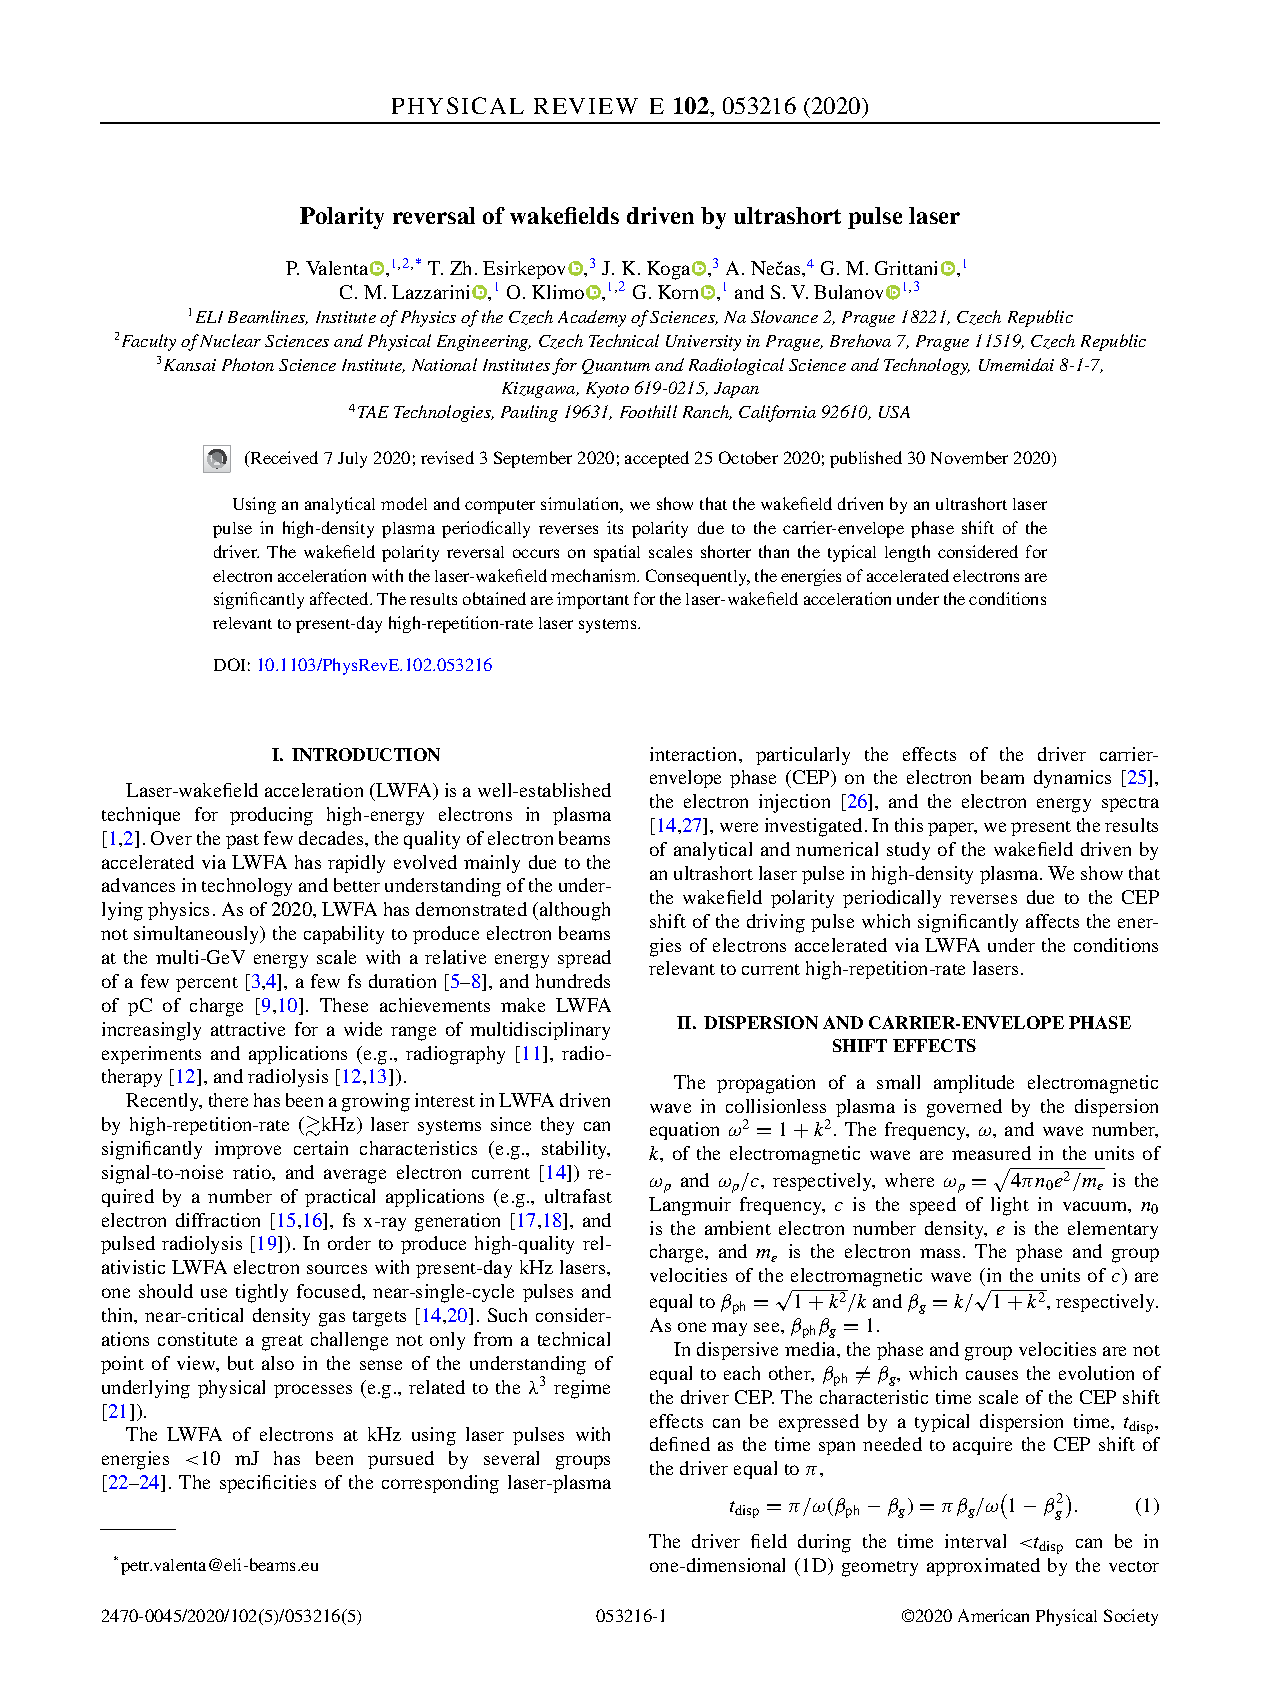
\includepdf[pages=-]{misc/paper2.pdf}

\mbox{}
\thispagestyle{empty}
\newpage

\section{Recoil effects on reflection from relativistic mirrors in laser plasmas \label{sec:paper_3}}

The following article is reproduced from Valenta, P., Esirkepov, T. Z., Koga, J. K., Pirozhkov, A. S., Kando, M., Kawachi, T., Liu, Y. K., Fang, P., Chen, P., Mu, J., Korn, G., Klimo, O., and Bulanov, S. V. (2020). \link{http://dx.doi.org/10.1063/1.5142084}{Recoil effects on reflection from relativistic mirrors in laser plasmas}., \textit{Physics of Plasmas}, \textbf{27}(3):032109, with the permission of AIP Publishing. \\

\noindent Copyright {\copyright} {2020} {American Institute of Physics}.

\newpage
\mbox{}
\thispagestyle{empty}

\newpage
\includepdf[pages=2-]{misc/paper3.pdf}

\section{Relativistic flying forcibly oscillating reflective diffraction grating \label{sec:paper_4}}

The following article is reproduced from Mu, J., Esirkepov, T. Z., Valenta, P., Gu, Y., Jeong, T. M., Pirozhkov, A. S., Koga, J. K., Kando, M., Korn, G., and Bulanov, S. V. (2020). \link{http://dx.doi.org/10.1103/PhysRevE.102.053202}{Relativistic flying forcibly oscillating reflective diffraction grating}. \textit{Physical Review E}, \textbf{102}(5):053202, with the permission of APS. \\

\noindent Copyright {\copyright} {2020} {American Physical Society}.

\newpage
\mbox{}
\thispagestyle{empty}

\newpage
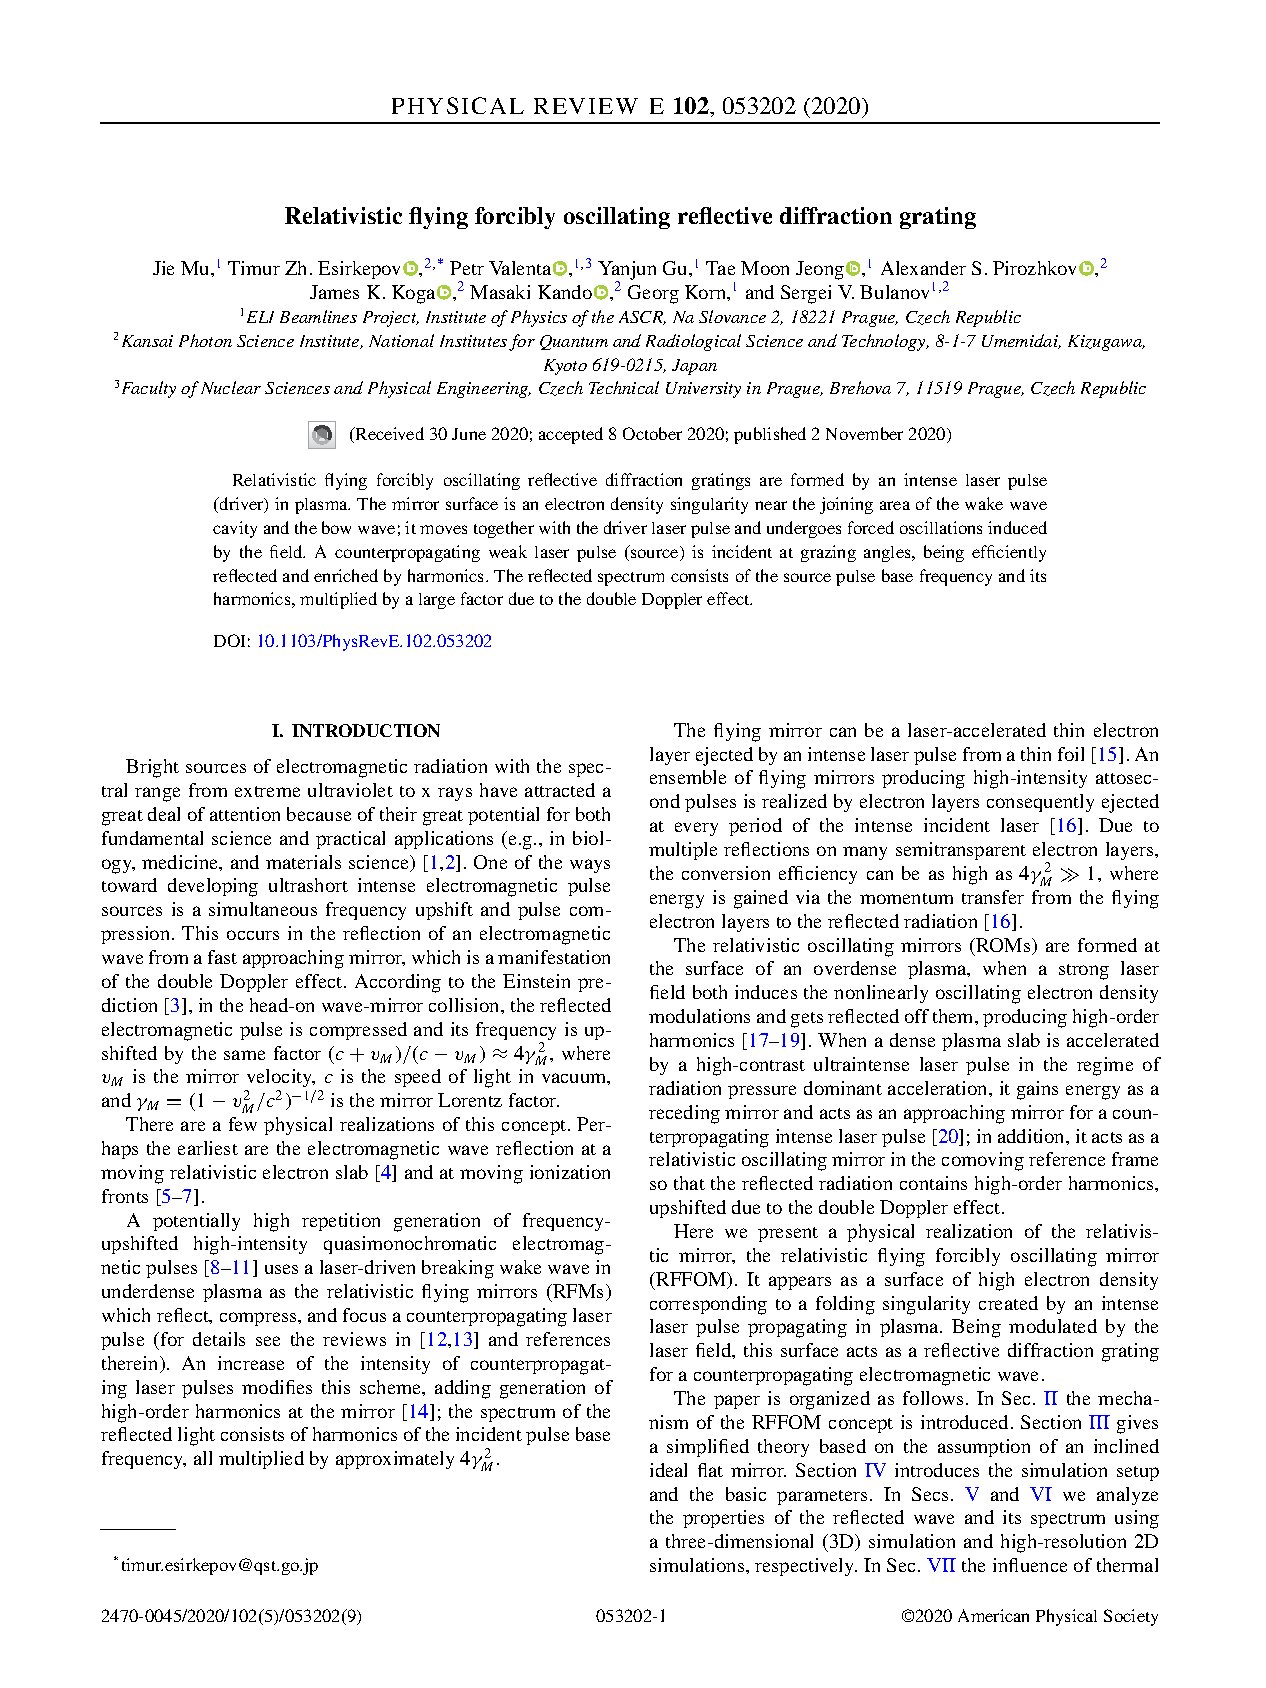
\includepdf[pages=-]{misc/paper4.pdf}

%\chapter{Code listings}
%\input{dat/appendix_b.tex}

%\chapter{CD content}
%\input{dat/appendix_c.tex}

\end{document}